\documentclass{dependencies/acm_proc_article-sp}

\usepackage{url}
\usepackage{color}
\usepackage{verbatim}
\usepackage{listings}
\lstset{
  language=C++,             % choose the language of the code
  basicstyle=\small,       % the size of the fonts that are used for the code
  numbers=left,                   % where to put the line-numbers
  numberstyle=\footnotesize,      % the size of the fonts that are used for the line-numbers
  stepnumber=0,                   % the step between two line-numbers. If it is 1 each line will be numbered
  numbersep=5pt,                  % how far the line-numbers are from the code
  backgroundcolor=\color{white},  % choose the background color. You must add \usepackage{color}
  showspaces=false,               % show spaces adding particular underscores
  showstringspaces=false,         % underline spaces within strings
  showtabs=false,                 % show tabs within strings adding particular underscores
  %frame=single,                   % adds a frame around the code
  tabsize=2,              % sets default tabsize to 2 spaces
  captionpos=t,                   % sets the caption-position to bottom
  breaklines=false,        % sets automatic line breaking
  breakatwhitespace=false,    % sets if automatic breaks should only happen at whitespace
  escapeinside={\%}{)}          % if you want to add a comment within your code
}

% Get rid of the permission block
\makeatletter
\let\@copyrightspace\relax
\makeatother

\begin{document}

%\title{ Distributed Systems: Project Description }
\title{ Distrivia: A Distributed Trivia Game }
\numberofauthors{3}
\author{
\alignauthor
Brian Gianforcaro \\
       \affaddr{Rochester Institue of Technology}\\
       \email{bjg1955@rit.edu}
\alignauthor
Steven Glazer \\
       \affaddr{Rochester Institue of Technology}\\
       \email{sfg6126@rit.edu}
\alignauthor
Samuel Milton \\
       \affaddr{Rochester Institue of Technology}\\
       \email{srm2997@rit.edu}
}
\maketitle

%\begin{abstract}
%In this paper we detail our current progress on our distributed trivia game.
%We will explain what has been done so far, what we need to do, and how we
%have met the requirements for the project. We also discuss the architecture
%for our system.
%\end{abstract}

\section {What We've Done}
Much of our system has been implemented and is in the debugging phase. The server apps, web client, and android client are nearly complete with some revisions happening as necessary. We have also started development on an application for the iPhone platform. The extent of what has been finished for each part of our system is explained below.

\subsection{Architecture Overview }
\begin{figure}[h!]
  \centering
    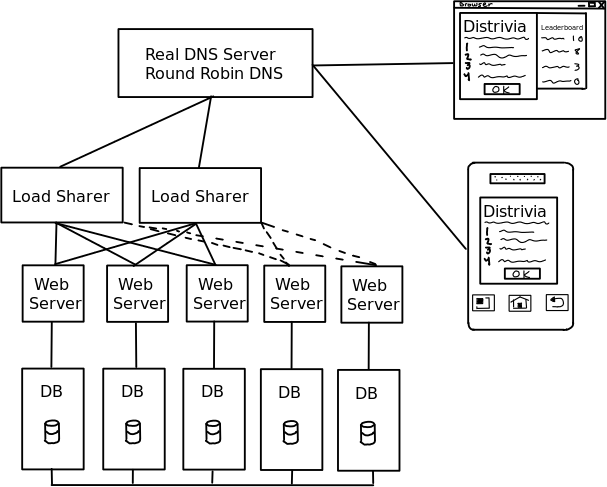
\includegraphics[scale=0.4]{diagram.png}
   \caption{High level overview of the system}
 \end{figure}

\subsection {Servers}
Currently, we have 6 servers running on Amazon's Elastic Compute Cloud \cite{aec}. One server is being used as a web-monitor
host. We are able to login to the web-monitor to see the status of all our
servers, databases, and load sharers. This will help us manage if the services
are running and allow us to track down any problems, if they arise. Three
servers are all running our server application and hosting the databases.
We also have two final servers that we have setup as hot spares in the event
of partial or total failure.
Each server contains the server application that responds to clients as well as
the Riak \cite{riak} databases. Riak auto-synchronizes the databases between the 5 servers.
Note that the hot spares are setup to be part of the database cluster so they
have a full copy of the database on hand, however they don't accept any reads
or writes directly. This allows for them to immediately be ready for read/writes in the event that the original servers are down.
With this configuration if we were to add a server, we would just need to update 
Riak and it would sync the databases to any additional servers as well. These servers,
therefore, all contain the same information. If any servers go down, the distributed
system would still run fine. We could have all servers go down except one and still
be reliably handling requests.

\subsection {Server Applications}
The server is currently almost feature complete, but still needs a lot of
testing. Client registration, and login are all supported. A client can
join a game, retrieve questions for that game, and answer questions. Both a
global leader board and individual per game leader board can also be requested.
We recently refactored our API to be more universally consistent.
The servers and clients now work on a more consistent basis where the clients all expect the same information and use the same calls.

\subsection {Traffic}
We have two load sharers set up. Both sharers are currently configured to
divide the requests among the three active servers and, if need be, the two hot spares. The duplicate sharers allow
for a load distributer to go down and we would still be able to serve requests
to the servers. These load sharers are selected by the clients using round
robin DNS where distrivia.lame.ws will select either load distributer that is
up at random. This provides us will stability for access to the servers. The
load sharers are setup to attempt to connect to a server twice before
deeming it dead and removing it from its list of servers to direct clients towards.
Currently we are using the NGINX \cite{nginx} in a reverse proxy configuration
for our load sharing needs.

\subsection {Clients}
Our focus for clients has been on a web-based client and an android application.
Both clients have most of the the workings completed. The web-based client will
be run from desktop platforms and laptop platforms. The android client will run
on any android phone running OS 2.1 or higher and does not use any unique services that require specific
hardware. Both clients are nearly fully-functional. They can, currently, login/register
players, view leaderboards, join public games, and compete in public games. We are actively adding features to both clients, daily.
We have also started development on an iPhone application for distrivia. This client does not yet communicate with the server, but 
it does implement nearly all the views seen in the other clients. We have been setting up the network communication for the iPhone
platform as well.

\subsection {Messages}
We are currently using the https protocol for our messages. This provides a secure
and usable messaging system that we have designed our client and server APIs to use.
The actual messages are sent and received in two way's. Initially a user session key is
generated using the UUID \cite{uuid} algorithm and returned to the user on successful
authentication. This session key is then passed back to the server with every in coming
message. Messages are sent to the server using POST and GET request methods supported
by the HTTP protocol. Responses from the server are in the form of JSON \cite{json} objects.
JSON is a small, easily parseable format, representing objects in a human readable format as
they would be represented in JavaScript. With the web client the JSON object returned from
the server is instantly usable, however for the android client we have to parse the JSON object
into a native Java object. The Android SDK provides libraries to do this, located in the
org.json \cite{orgjson} package name space.



\section {What's Left}
\subsection {Server}
The server is nearly completed. The server application just needs to have some tweaks and further testing.
\subsection {Web Client}
A lot of the main features of the web client are completed.
However, there are still a few remaining features that need to be implemented.
While private games are implemented on the server, 
Also, when a user clicks on a button to do something like log in, the button should be disabled while waiting for a response,
alternatively it needs to be able to handle sending out two calls for the same request and not getting confused if it gets two back.
\subsection {Android}
Private gameplay is the largest thing left for the android client. Besides this we've just been fixing bugs and cleaning up the UI.
\subsection {iPhone}
The iPhone application just started development in the last couple days. We have built most of the UI but need to connect all of the actions
to the server. We will need to implement everything, including login/registration, joining public/private games, viewing leaderboards,
and competing in rounds.

\section {Meeting the Requirements}

Our system has three unique clients. One of them is designed for the Android platform as an app.
Another is designed for the iPhone platform as a native app.
The third is a web client, which is specifically being tested on Desktop and Laptop
browsers, however it may work on many hand held web browsers as well.

Our system supports having any number of servers and allowing any subset of them to fail.
We are using Riak, which supports a 'shared nothing' architecture.  We can add a new server
by joining it to our database and starting the web server.  This can be done as many times
as needed, allowing us to scale up our system.  These same principles also give us great fault
tolerance, since any server is capable of running independently.  As long as one server is still
up, the service will be available.

We use round robin DNS to allow our clients to be completely ignorant of our servers.  Load sharers
can be added and removed from the DNS server and the clients will be completely ignorant of this
and unaffected.  The load sharers in turn know about our data servers and do their best to
distribute the load across them.  When a new server is added, it is just added to our load sharer
configuration file and clients can start using it.  When a server fails, the sharers will stop directing
traffic to it.


We are currently using Riak as our database backend. We chose Riak for multiple
reasons, but the biggest was it's focus on  scalability, fault-tolerance,
availability, and replication. Riak is a Amazon Dynamo \cite{dynamo} inspired
database, it supports full masterless replication. In Riak every node can
serve client requests and they are propagated to the rest of the cluster.
In our system we have made sure that this replication occurs between nodes
on Amazon EC2's internal Gigabit ethernet so it is as fast as possible. Riak
also has the unique property that if all of the nodes but one fail, the single
node can still accept both reads and writes to the database. When the other
nodes return to operational state from failure, all changes will automatically
be propagated to all of the nodes. This feature is the basis for our ability to
support and recover from partial failures. In the event that two Riak nodes accept
writes from two separate clients modifying the same data and Riak is unable
to resolve the conflict the user is given both versions and allowed to resolve
the conflict them selves. However we have configured our installation so this
can not occur, we have specified that every available node must agree on a
write before it is committed. Given the relatively small number of nodes (five)
that will take part in this agreement, we decided that the possible overhead
was acceptable for the increased level of consistency it gives us.

Our team is taking a very proactive stance towards security. All of our machines are properly firewalled so that
outside clients can not authenticate to our database cluster. Also we have implemented SSL through our entire infrastructure.
Our load sharer's automatically redirect http:// to https:// and once you are in https:// at the load sharer, SSL continues all the
way back to our actual web application back end serving responses over a SSL wrapped socket. This way no passwords are ever
sent in clear text. Our group even found a SSL certificate authority who was willing to sign our SSL certificate for free. This gives
us actual fully functional, authenticatable SSL infrastructure. In order to make sure that our system properly secures user information,
we stuck with the industry standard of storing a hashed version of the users password instead of the password itself. We decided on using
the cryptographically secure hashing function designed for passwords known as bcyrpt \cite{bcrypt}.

\newpage
%
% The following two commands are all you need in the
% initial runs of your .tex file to
% produce the bibliography for the citations in your paper.
\bibliographystyle{abbrv}
\bibliography{bibliography}  % sigproc.bib is the name of the Bibliography in this case
% You must have a proper ".bib" file
%  and remember to run:
% latex bibtex latex
% to resolve all references
%
% ACM needs 'a single self-contained file'!
%
%APPENDICES are optional
\balancecolumns
% That's all folks!
\end{document}
